% Template for ICME-2010 paper; to be used with:
%          spconf.sty  - ICASSP/ICIP LaTeX style file, and
%          IEEEbib.bst - IEEE bibliography style file.
% --------------------------------------------------------------------------
\documentclass{article}
\usepackage{spconf_ICME,amsmath,epsfig,fancyhdr}
\setlength{\paperwidth}{215.9mm} \setlength{\hoffset}{-9.7mm}
\setlength{\oddsidemargin}{0mm} \setlength{\textwidth}{184.3mm}
\setlength{\columnsep}{6.3mm} \setlength{\marginparsep}{0mm}
\setlength{\marginparwidth}{0mm} \setlength{\paperheight}{279.4mm}
\setlength{\voffset}{-7.4mm} \setlength{\topmargin}{0mm}
\setlength{\headheight}{0mm} \setlength{\headsep}{0mm}
\setlength{\topskip}{0mm} \setlength{\textheight}{235.2mm}
\setlength{\footskip}{12.4mm} \setlength{\parindent}{1pc}

\usepackage{minted}

\ICMEfinalcopy % *** Uncomment this line for the final submission

\def\ICMEPaperID{****} % *** Enter the ICME Paper ID here
\def\httilde{\mbox{\tt\raisebox{-.5ex}{\symbol{126}}}}

% Pages are numbered in submission mode, and unnumbered in camera-ready
\ifICMEfinal\pagestyle{empty}\fi


\begin{document}\sloppy

% Example definitions.
% --------------------
\def\x{{\mathbf x}}
\def\L{{\cal L}}


% Title.
% ------
\title{Using N-gram similarity metrics for Relation Clustering}
%
% Single address.
% ---------------
\name{Stephen Mayhew, Nicholas Kamper}

\address{
\textit{mayhewsw@rose-hulman.edu}\\
\textit{kampernj@rose-hulman.edu}\\
Rose-Hulman Institute of Technology}


\maketitle
% insert page header and footer here for IEEE PDF Compliant
\thispagestyle{fancy} \fancyhead{} \lhead{}
\lfoot{\copyright2012 SWM, NJK} \cfoot{}
%\rfoot{ICME 2010}
\renewcommand{\headrulewidth}{0pt}
\renewcommand{\footrulewidth}{0pt}


%
%\begin{abstract}
%This paper has to do with relation extraction. This is probably best written %after the rest of the paper is done.
%\end{abstract}
%
%\begin{keywords}
%Natural Language Processing, Information Extraction, Relation Extraction, %Coreference Resolution
%\end{keywords}
%
\section{Introduction}
\label{sec:intro}

The overall goal of our project was to use Hidden Markov Models (HMM) to cluster relations. A relation is a triple of the form (object, relation, object), such as \textit{(george washington, was president of, the usa)}. Such relations are the output of relation extractors. These relation extractors process a massive amount of web text, and inevitably produce many different strings that refer to the same thing. The goal of this system is to cluster these extractions by their meaning. For example, one such cluster might be:

\fvset{frame=single}
\begin{minted}[fontsize=\footnotesize]{text}
(tony blair, is prime minister of, britain) 
(tony blair, is prime minister of, great britain) 
(tony blair, is the prime minister of, the UK)
\end{minted}
\fvset{frame=none}

We note that facts do not need to be true to be part of the system.



\section{Project Background}
We began by looking into ways that HMMs could be used to solve the problem. Our thought process went: we will need to compare every sentence against every other to check similarity. We can train an HMM on a given sentence, and then test every other sentence on that HMM. The resulting score would be compared to some threshold in order to decide if those two strings should be clustered. 

This approach had many problems. First of all, that is a fragile model (how to deal with skips etc.). Second, one sentence does not train very well. 

Another line of thought was, perhaps the hidden states are meanings, and the text is an output. This was a good thought, but there is no limit on the number of meanings, and no limit on the number of outputs. 


HMM for scoring (Multiple sequence alignment). Dead wall.
Next we researched using a technique called Multiple Sequence Alignment, which is used in biological research to classify protein sequences. This seemed promising to begin with, but we realized that the domain of the protein alphabet is much smaller (4 symbols), and this caused problems for us. 

Having failed these two applications, we were at a loss. It seemed that HMMs may not be the best tool for the job.

Our next exploration focused on n-gram models. It seemed reasonable to use n-gram models in a similar way as described for HMM's above: when comparing every pair of strings, we create an n-gram model using the first string, and test it with the second one. Unsurprisingly, this failed for many of the same reasons. The scores it returned were largely erratic and useless. That is, it would classify strings as ``microsoft windows'' as being more likely to match ``barack obama'' than ``president obama'' would be. We were using NLTK, which in turn used n-gram models with Katz backoff, and Lidstone smoothing \cite{nltk}. 

Since we also had 87-GB of Google n-gram data at hand, we considered how we could use it. However, we could not find any good way to use it.

Before we landed on using NLTK, we tried several different libraries, including OpenNLP, KYLM. These, however, were either only partially implemented, or only partially documented. We found them to be of little help.

Finally, we chanced on Python n-gram similarity library that uses n-grams to predict similarity between two strings. This library is given the imaginative name of ``NGram". The documentation describes it as follows: ``The NGram class is a set that supports searching for its members by N-Gram string similarity." \cite{py_ngram_lib}





What kind of results did we get?

What are we going to try to get better results?


\section{N-Gram Similarity Model, Our Clustering}
We examined the Python NGram string similarity library to understand how it works. It is a single file, and it took less than half an hour to read it through. We summarize the algorithm in Figure \ref{algorithm}.

Our clustering algorithm is a very simple $\mathcal{O}(n^2)$ algorithm, outlined in Figure \ref{clustering}.

\begin{figure}
\fvset{frame=single}
\begin{minted}[mathescape,fontsize=\footnotesize,tabsize=4]{python}
def compare(string: s1, string: s2, int: N):
	s1_padded = pad s1 on either side using
				   N-1 padding characters.
	s1_ngrams = split s1_padded into n-grams 
				   of length N
	
	s2_padded = pad s2 on either side using
				   N-1 padding characters.
	s2_ngrams = split s2_padded into n-grams 
				   of length N	
	
	samegrams = intersection of s1_ngrams
			 	   & s2_ngrams
	
	allgrams = len(s1_ngrams) + len(s2_ngrams)
			  	  - len(samegrams)
	
	return samegrams / allgrams
\end{minted}
\fvset{frame=none}
\vspace{-20pt}
\caption{N-gram Similarity Algorithm}
\label{algorithm}
\end{figure}

\begin{figure}
\fvset{frame=single}
\begin{minted}[mathescape,fontsize=\footnotesize,tabsize=4]{python}
def cluster(string []: extractions as e):
	threshold = some value
	N = some value

	for i in range(len(e)):
		for j in range(i+1, len(e)):
			score = compare(e[i], e[j], N)
			
			if score > threshold:
				cluster e[i] and e[j]
\end{minted}
\fvset{frame=none}
\vspace{-20pt}
\caption{Our Clustering Algorithm}
\label{clustering}
\end{figure}


\section{Experiments}
For each experiment, we wrote a script that could run the clusterer multiple times but with different parameters. The two parameters we changed were N, the length of the n-grams, and the threshold, as used in Figure \ref{clustering}.




Baseline - easy.

Backoff - between two different strings, if no ngrams matched, then try again 
with N being one less.

The idea being that we would not accept 0 as an answer. 0 is not a very useful answer.

Cumulative data - as follows:
N = high number
score = 0
while N > 1:
	score += compare with N
 	N = N-1 

The idea being that strings with several long n-grams in common should be given credit. 


Extending the model: we match strings by every string in the cluster so far. 
The problem with this approach was that as soon as a wrong string was added to a cluster, it opened the door for a large number of other bad strings. With various experiments with the threshold, we found that it had a way of either putting all strings in one big cluster, or separating each string into it's own one-element cluster. 

How about a variable threshold for extending the model? This could also work. The idea would be to have a very strict threshold at first, so only similar strings would be added. But as more strings are added, raise the threshold so that it is not so stringent any more. How does this work?





\section{Results}
The F1 measure is a combination of precision and recall. The F1 measure is a percentage. 

About 70\% F1 measure in the best cases.

We found that the baseline results (see Figure \ref{baseline}) were as good or better than any of the experiments we tried.

The results for backoff (see Figure \ref{backoff}) were slightly worse, but more consistently better.

\begin{figure}
\begin{center}
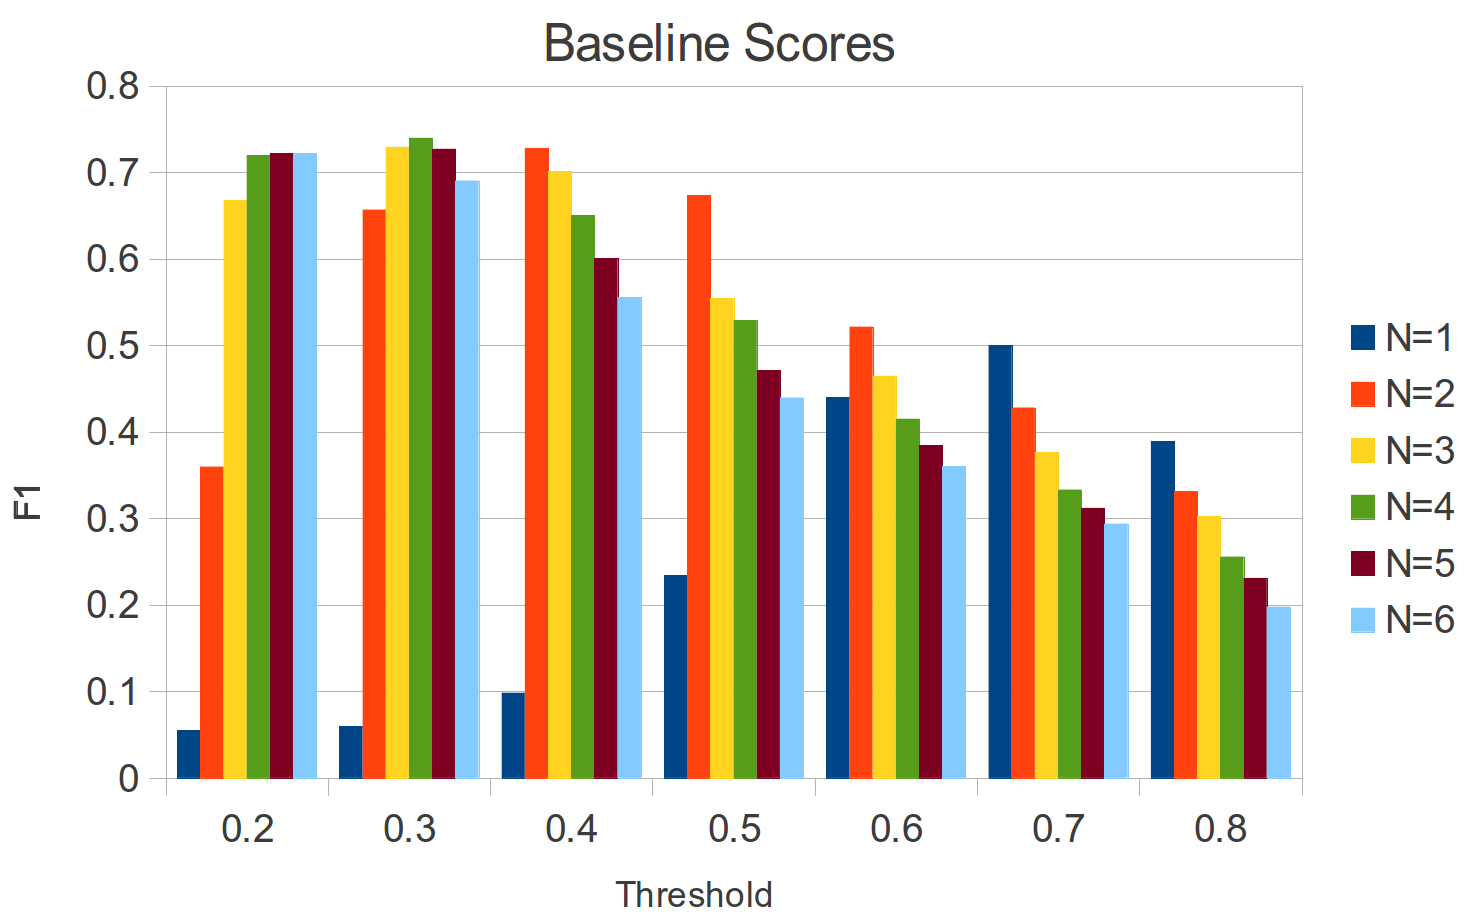
\includegraphics[scale=0.17]{baselinescores.png}
\end{center}
\caption{Baseline Results}
\label{baseline}
\end{figure}


\begin{figure}
\begin{center}
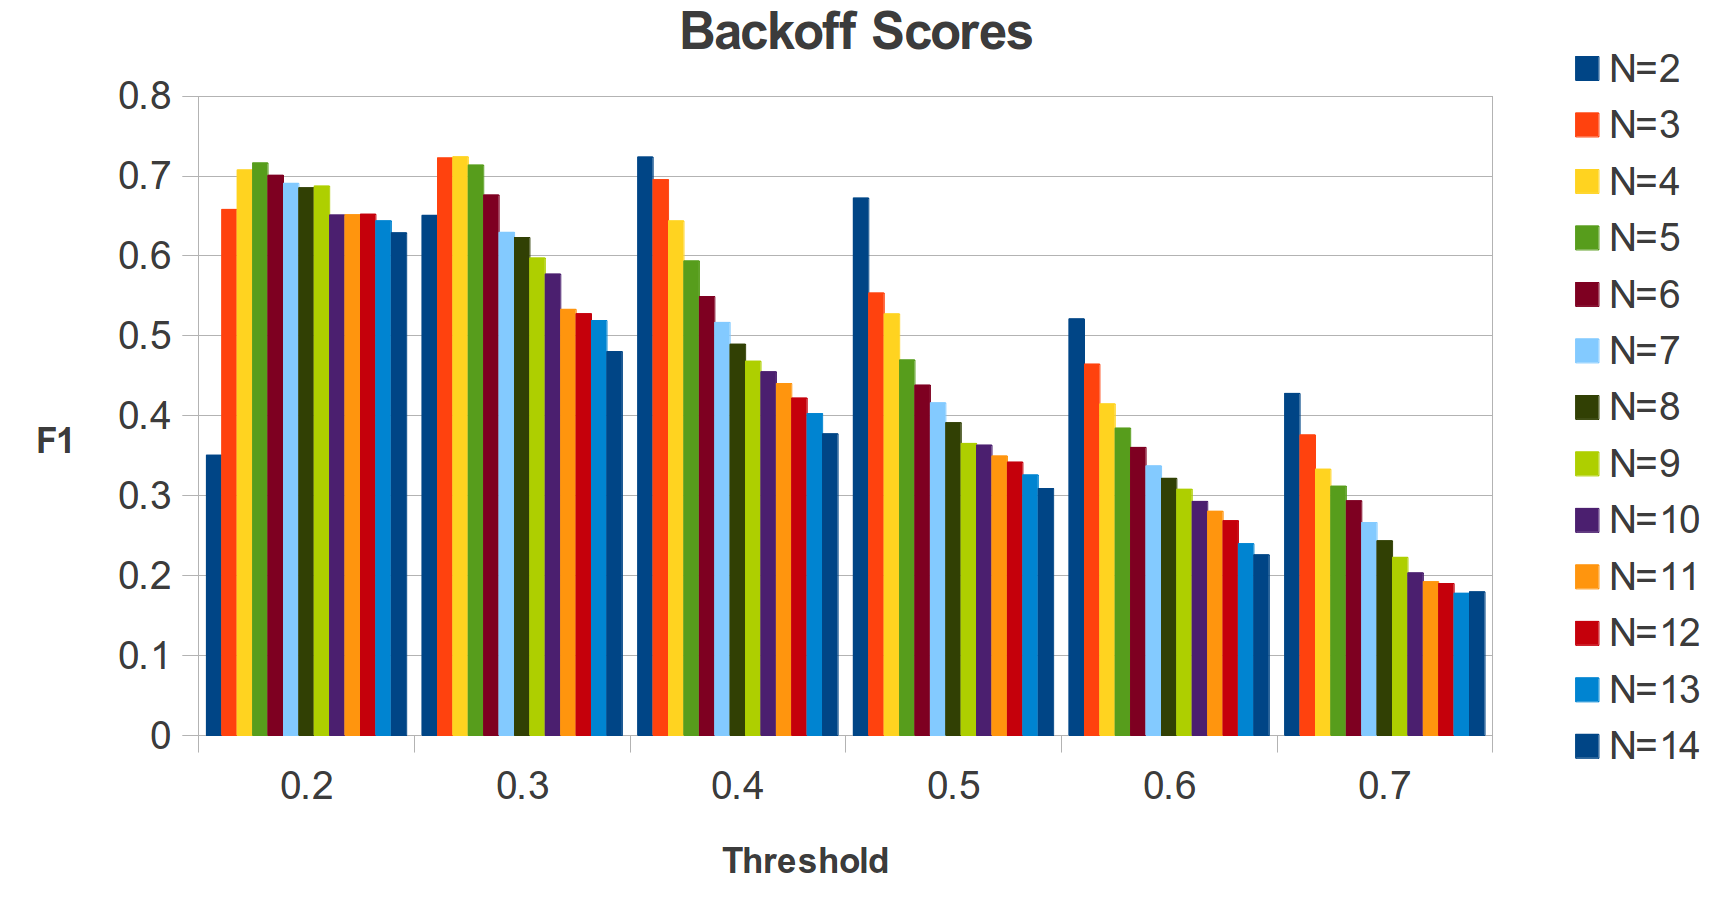
\includegraphics[scale=0.17]{backoff.png}
\end{center}
\caption{Backoff Results}
\label{backoff}
\end{figure}


\section{Future Work}
look into techniques outlined in \cite{ngram_sim}








Possibility: backing off. (just reduce N)

\begin{thebibliography}{1}

\bibitem{py_ngram_lib}
Michel Albert, Graham Poulter, and open source contributors. Python NGram Similarity Library. \textit{http://packages.python.org/ngram/}

\bibitem{yates2009}
Alexander Yates, Oren Etzioni (March, 2009). \textit{Unsupervised Methods for Determining Object and Relation Synonyms on the Web}. Journal of Artificial Intelligence Research (JAIR). 

\bibitem{nltk}
Bird, Steven, Edward Loper and Ewan Klein (2009). \textit{Natural Language Processing with Python}.  O'Reilly Media Inc.

\bibitem{ngram_sim}
Kondrak, Grzegorz (2005). \textit{N-gram similarity and distance}. In Proceedings of the 12th International Conference on String Processing and Information Retrieval (Buenos Aires, Argentina). 115–126.

\end{thebibliography}


\end{document}